\documentclass[aspectratio=169,8pt]{beamer}  % Reduced base font size to 8pt

% Theme settings
\usetheme{metropolis}
\usecolortheme{default}
\usepackage[utf8]{inputenc}
\usepackage{graphicx}
\usepackage{amsmath}
\usepackage{booktabs}

% Theme and color settings
\definecolor{background}{RGB}{255,255,255}
\setbeamercolor{background canvas}{bg=background}
\setbeamercolor{normal text}{fg=black}
\setbeamercolor{frametitle}{bg=background, fg=black}
\setbeamercolor{title}{fg=black}
\setbeamercolor{subtitle}{fg=black}
\setbeamercolor{section title}{fg=black}
\setbeamercolor{footline}{fg=black, bg=background}
\setbeamercolor{block title}{bg=gray!15,fg=black}
\setbeamercolor{block body}{bg=white,fg=black}

% Font size adjustments
\setbeamerfont{frametitle}{size=\small}
\setbeamerfont{title}{size=\Large}
\setbeamerfont{subtitle}{size=\normalsize}
\setbeamerfont{author}{size=\small}
\setbeamerfont{date}{size=\small}
\setbeamerfont{block title}{size=\small}
\setbeamerfont{itemize/enumerate body}{size=\small}
\setbeamerfont{itemize/enumerate subbody}{size=\footnotesize}

% Title info
\title{Visual Intelligence: Lung Cancer Histopathological Classification}
\author{Lorenzo Mioso}
\date{March 2025}

\begin{document}

% Title slide
\begin{frame}
\titlepage
\end{frame}

% Introduction slide with adjusted image alignment
\begin{frame}{Introduction \& Problem Statement}
\begin{columns}[T]
\begin{column}{0.5\textwidth}
\begin{itemize}
\item \textbf{Dataset}: Lung cancer histopathological images (3 classes):
  \begin{itemize}
  \item \textbf{Adenocarcinoma}
  \item \textbf{Squamous cell carcinoma}
  \item \textbf{Benign tissue}
  \end{itemize}
\item \textbf{Classification Task}: \textbf{Binary classification} (adenocarcinoma vs benign)
\item \textbf{Challenge}: Distinguishing \textbf{subtle tissue patterns} and \textbf{cellular structures}
\end{itemize}
\end{column}
\begin{column}{0.5\textwidth}
\hfill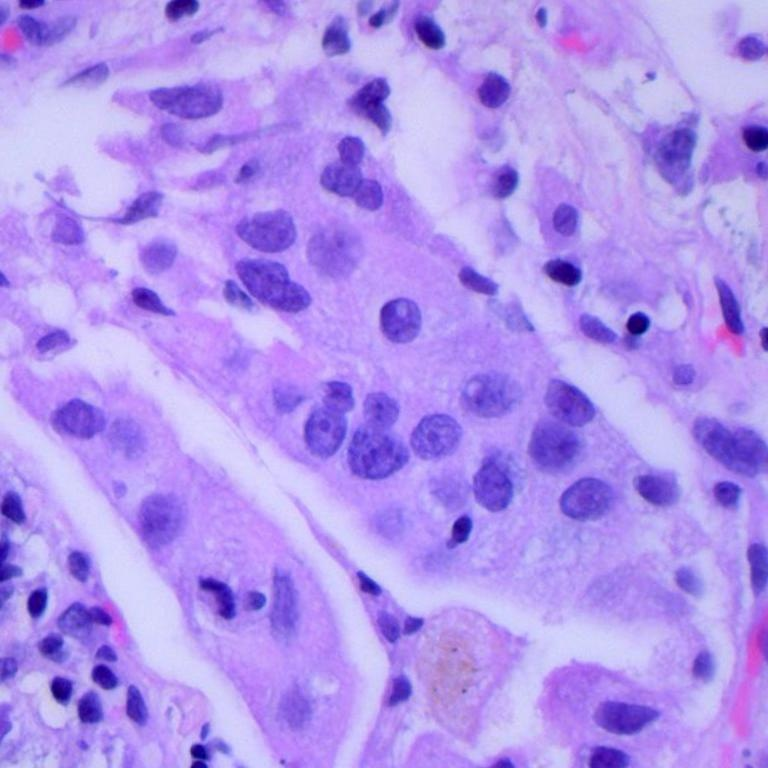
\includegraphics[width=0.95\linewidth, height=0.45\textheight]{imgs/adenocarcinoma.jpg}
\vspace{0.2cm}
\hfill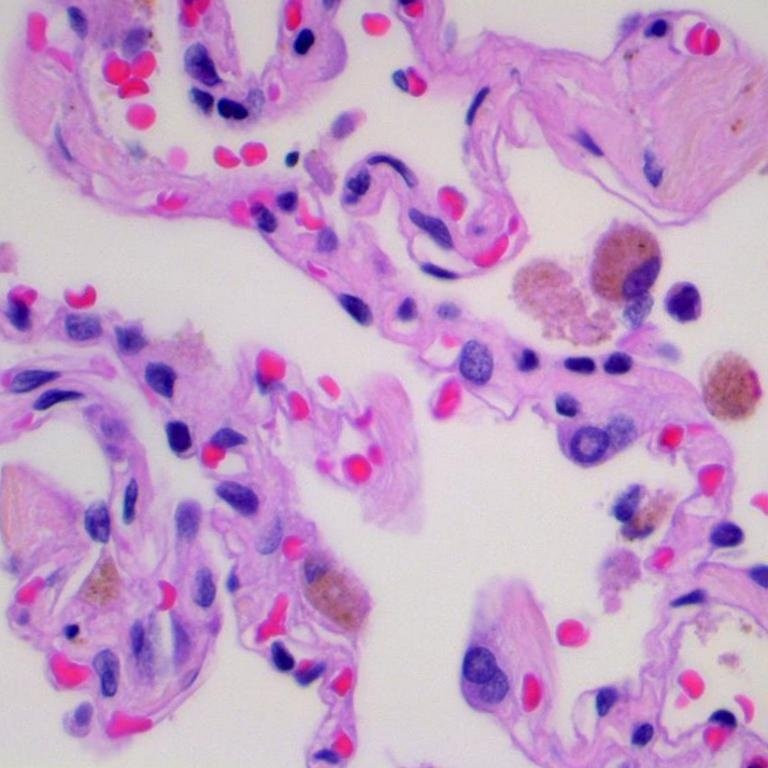
\includegraphics[width=0.95\linewidth, height=0.45\textheight]{imgs/benign.jpg}
\end{column}
\end{columns}
\end{frame}

% Project Goals slide
\begin{frame}{Project Goals}
\begin{itemize}
\item Compare \textbf{traditional CNN} vs \textbf{ScatNet} approaches
\item Investigate \textbf{color} vs \textbf{structural features}
\item Achieve \textbf{high accuracy} with \textbf{interpretable results}
\item Apply \textbf{explainable AI techniques} to validate model decisions
\end{itemize}
\end{frame}

% Data Preprocessing slide
\begin{frame}{Data Preprocessing \& Setup}
\begin{columns}[T]
\begin{column}{0.6\textwidth}
\begin{itemize}
\item \textbf{Dataset Organization}:
  \begin{itemize}
  \item \textbf{K-fold cross-validation} with 10 folds
  \item Class distributions already balanced
  \item Image size kept at \textbf{768×768 pixels}
  \item \textbf{Grayscale conversion} for analysis
  \end{itemize}
\end{itemize}

\begin{block}{Key Finding}
Using grayscale images for analysis because with only color images, the model achieved high accuracy by learning \textbf{color distributions}
\end{block}
\end{column}
\begin{column}{0.4\textwidth}
\begin{figure}
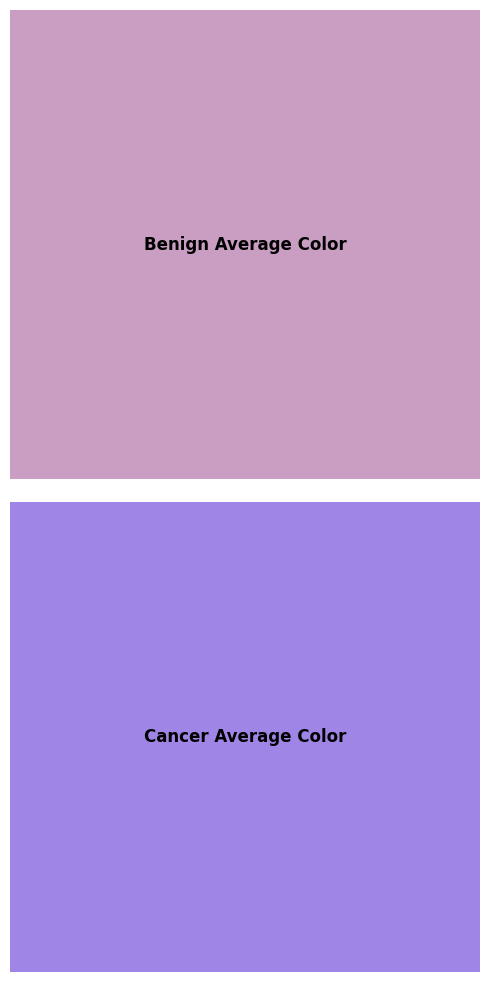
\includegraphics[width=0.7\textwidth, height=0.70\textheight]{imgs/class_avg_colors.png}
\end{figure}
\end{column}
\end{columns}
\end{frame}

% Preprocessing Pipeline slide with adjusted image alignment
\begin{frame}{Preprocessing Pipeline}
\begin{columns}[T]
\begin{column}{0.5\textwidth}
\begin{itemize}
\item Image \textbf{normalization} and \textbf{standardization} for each fold
\item Data augmentation decisions:
  \begin{itemize}
  \item Random rotations
  \item Random flips
  \item Color jittering
  \item Random cropping
  \item Gaussian noise
  \end{itemize}
\end{itemize}
\end{column}
\begin{column}{0.5\textwidth}
\hfill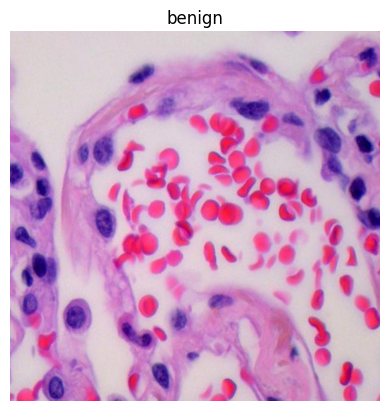
\includegraphics[width=0.95\linewidth, height=0.45\textheight]{imgs/normal_image.png}
\vspace{0.2cm}
\hfill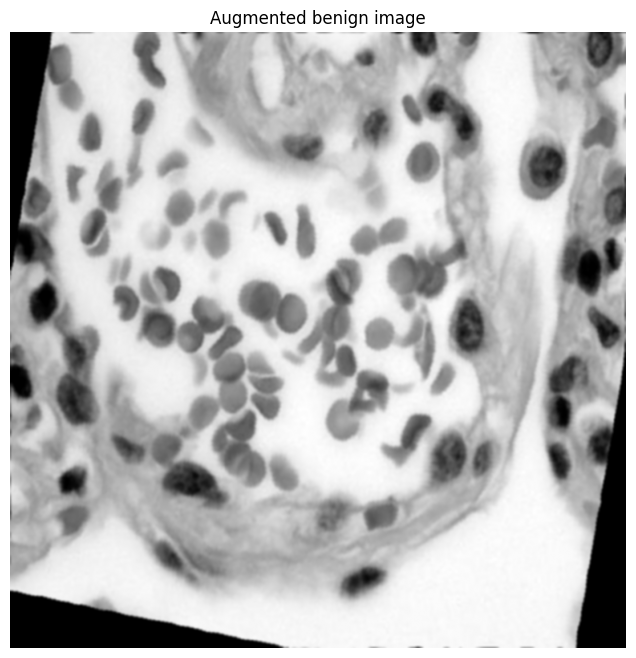
\includegraphics[width=0.95\linewidth, height=0.45\textheight]{imgs/augmented_image.png}
\end{column}
\end{columns}
\end{frame}

% CNN Model Architecture
\begin{frame}{CNN Model Architecture}
\begin{columns}[T]
\begin{column}{0.6\textwidth}
\begin{itemize}
\item \textbf{Efficient Feature Extraction Design}:
  \begin{itemize}
  \item Similar to \textbf{ResNet architecture} without skip connections
  \item Three progressive convolutional blocks (16→16→24)
  \item First convolutional layer with \textbf{11×11 kernel}
  \item Strategic dimensionality reduction via \textbf{max pooling}
  \item \textbf{Batch normalization} for improved training stability
  \item \textbf{ReLU activations} for non-linear patterns
  \end{itemize}
\end{itemize}

\begin{block}{Key Findings}
\begin{itemize}
\item Achieves \textbf{exceptional classification accuracy} despite minimal parameters
\item First layer filters may not appear visually interpretable with small learning rates
\end{itemize}
\end{block}
\end{column}
\begin{column}{0.4\textwidth}
\begin{figure}
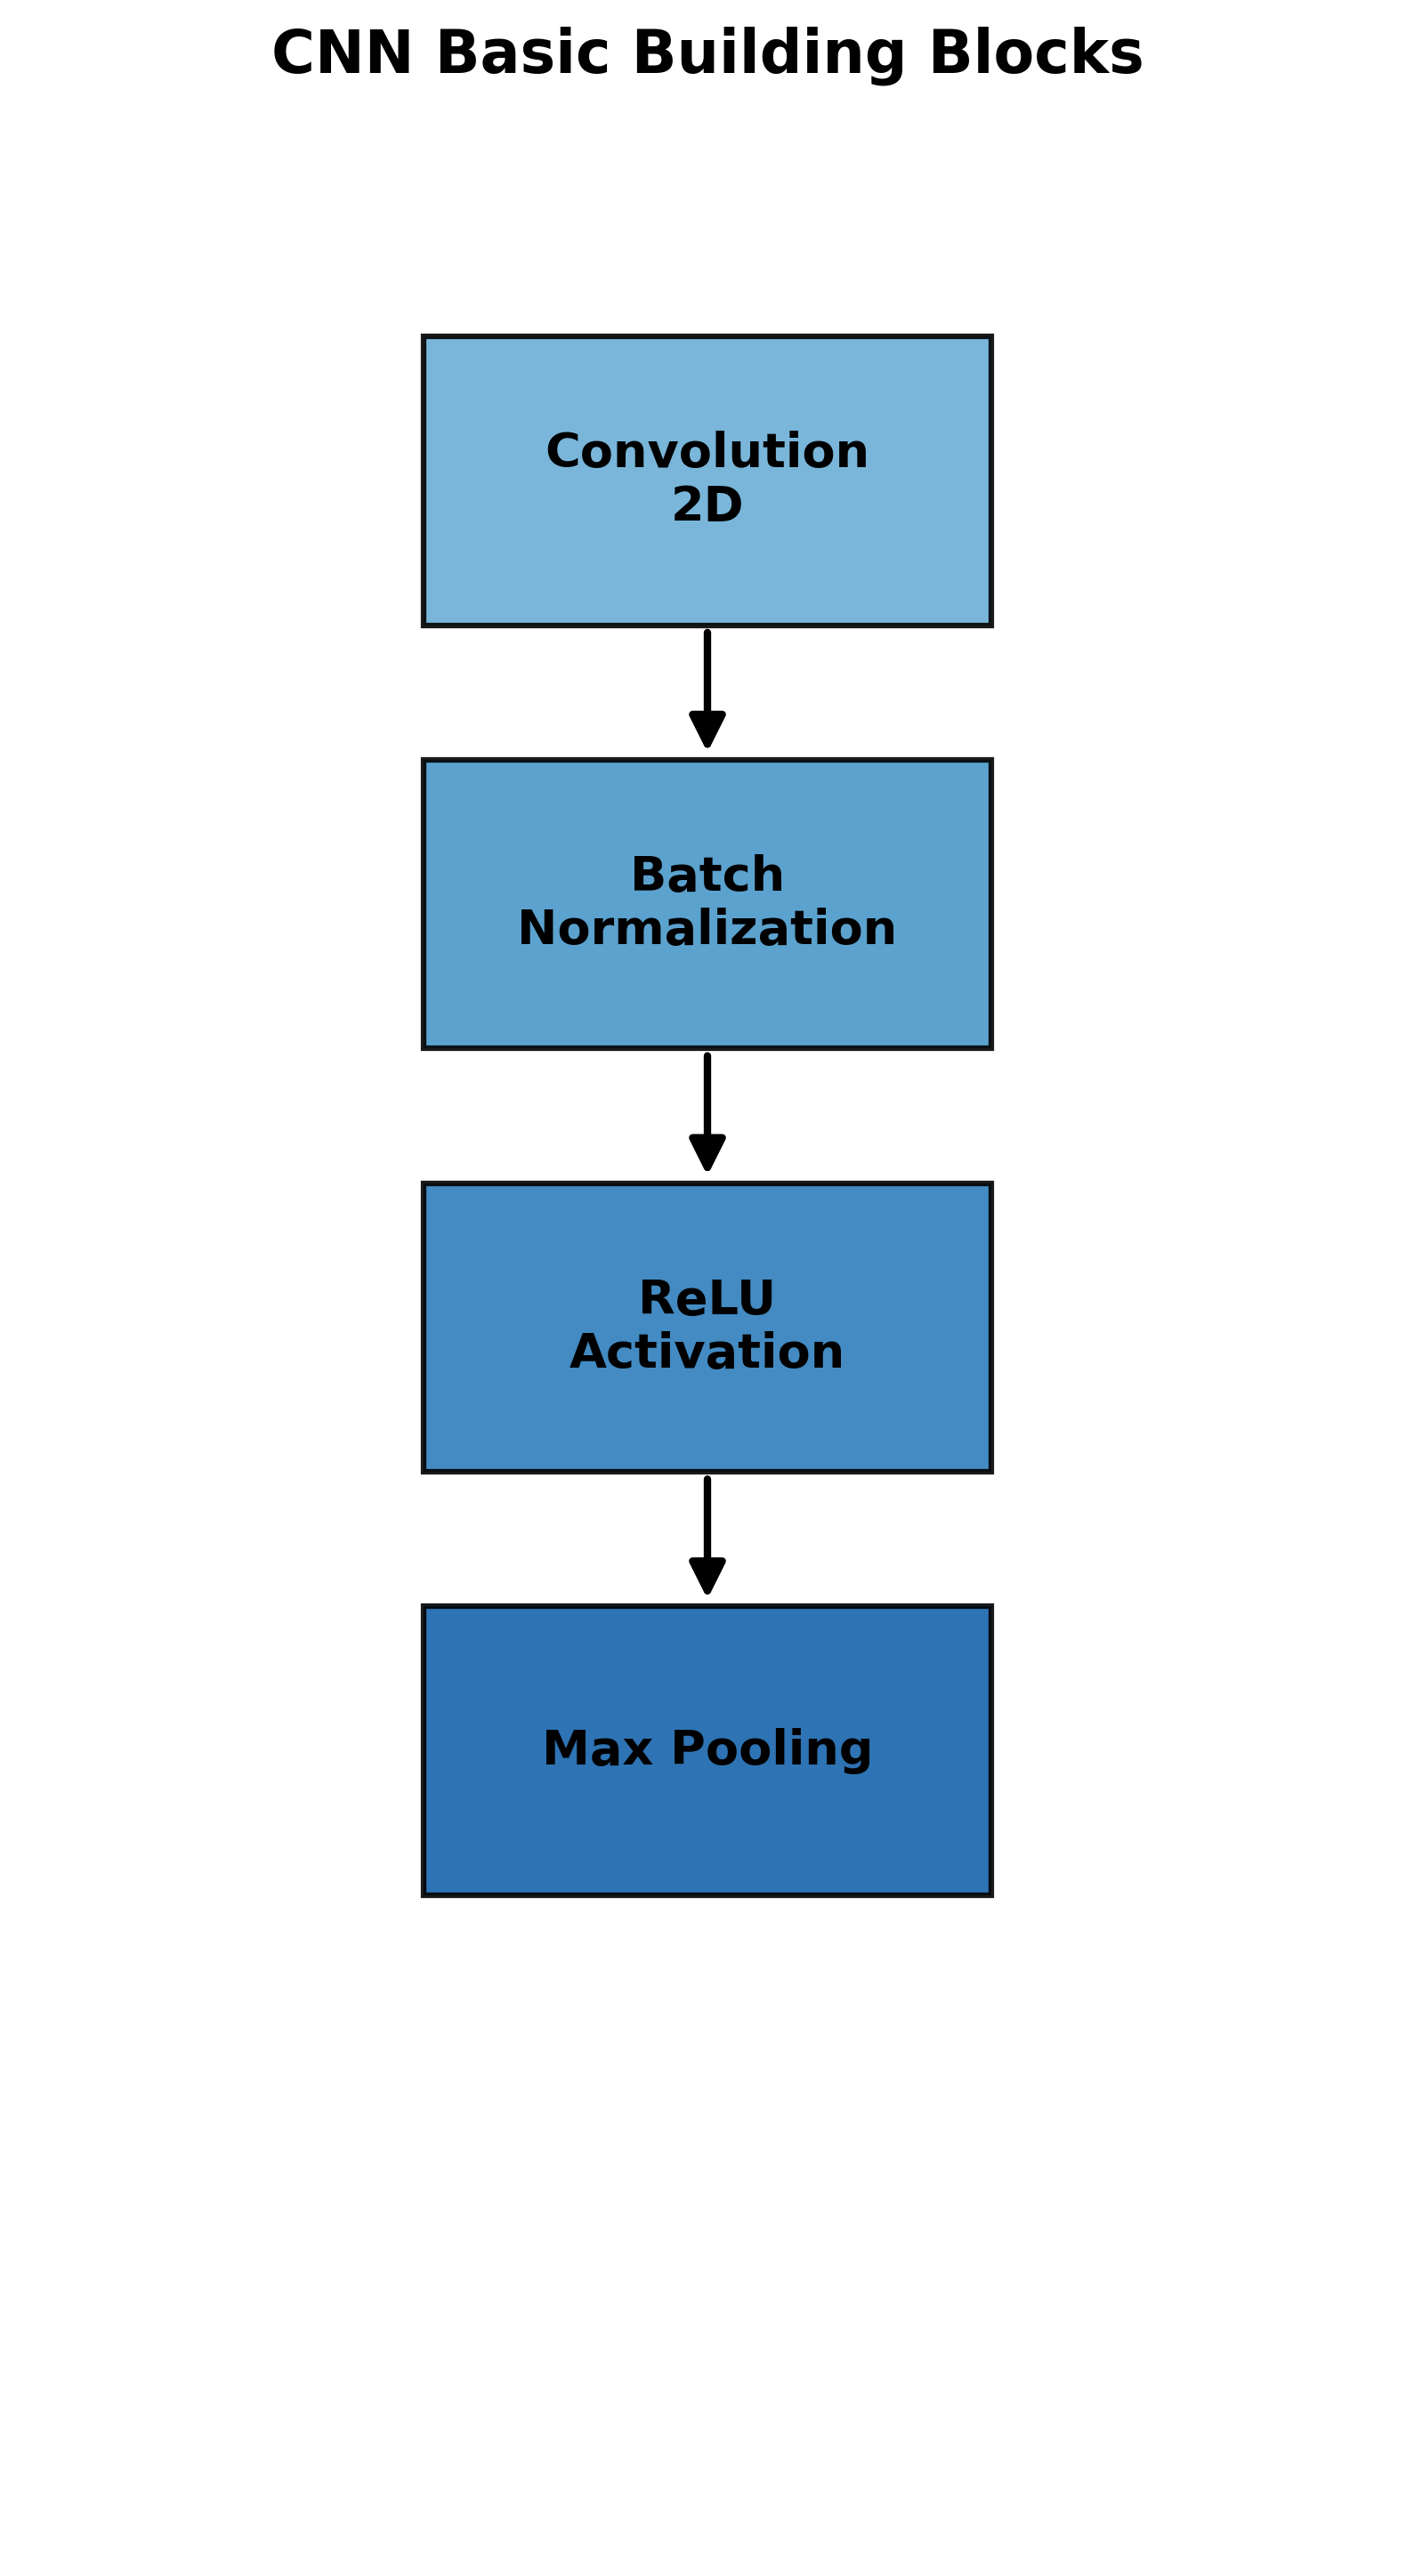
\includegraphics[width=0.9\textwidth]{imgs/cnn_basic_block.png}
\end{figure}
\end{column}
\end{columns}
\end{frame}

% CNN Architecture Details slide
\begin{frame}[fragile]{CNN Architecture Details}
\begin{columns}[T]
\begin{column}{0.6\textwidth}
\begin{verbatim}
CNNImageClassifier(
  (features): Sequential(
    (0): Conv2d(1, 16, kernel_size=(11, 11), stride=(2, 2))
    (1): BatchNorm2d(16)
    (2): ReLU()
    (3): MaxPool2d(kernel_size=2, stride=2)
    ...
  )
  (classifier): FeatureClassifier(
    (fc1): Linear(384, 16)
    (bn): BatchNorm1d(16)
    (relu): ReLU()
    (do): Dropout(p=0.5)
    (fc2): Linear(16, 2)
  )
)
\end{verbatim}
\end{column}
\begin{column}{0.4\textwidth}
\begin{itemize}
\item Total parameters: \textbf{14,090}
\item Model size: \textbf{52.58MB}
\item \textbf{Efficient architecture} with minimal parameters
\end{itemize}
\end{column}
\end{columns}
\end{frame}

% ScatNet Architecture slide
\begin{frame}[fragile]{ScatNet Model Architecture}
\begin{columns}[T]
\begin{column}{0.6\textwidth}
\begin{verbatim}
ScatNetImageClassifier(
  (scattering): Scattering2D()
  (global_pool): AdaptiveAvgPool2d(4, 4)
  (classifier): FeatureClassifier(
    (fc1): Linear(3472, 16)
    ...
  )
)
\end{verbatim}
\end{column}
\begin{column}{0.4\textwidth}
\begin{itemize}
\item \textbf{Wavelet-based feature extraction}:
  \begin{itemize}
  \item \textbf{J=3} scale parameter for wavelet decomposition
  \item \textbf{L=8} orientations, \textbf{M=2} scattering order
  \item \textbf{Translation}, \textbf{rotation}, and \textbf{scaling invariant}
  \end{itemize}
\end{itemize}

\begin{block}{Key Finding}
Requires \textbf{more complex classifier} layer for good performance
\end{block}
\end{column}
\end{columns}
\end{frame}

% Learning Curves Analysis slides
\begin{frame}{CNN Learning Curves Analysis}
\begin{columns}[T]
\begin{column}{0.5\textwidth}
\begin{itemize}
\item \textbf{Rapid convergence} within 15 epochs
\item \textbf{Consistent performance} across folds
\item \textbf{Limited overfitting} due to effective regularization
\item Final validation accuracy around \textbf{99\%}
\end{itemize}
\end{column}
\begin{column}{0.5\textwidth}
\begin{figure}
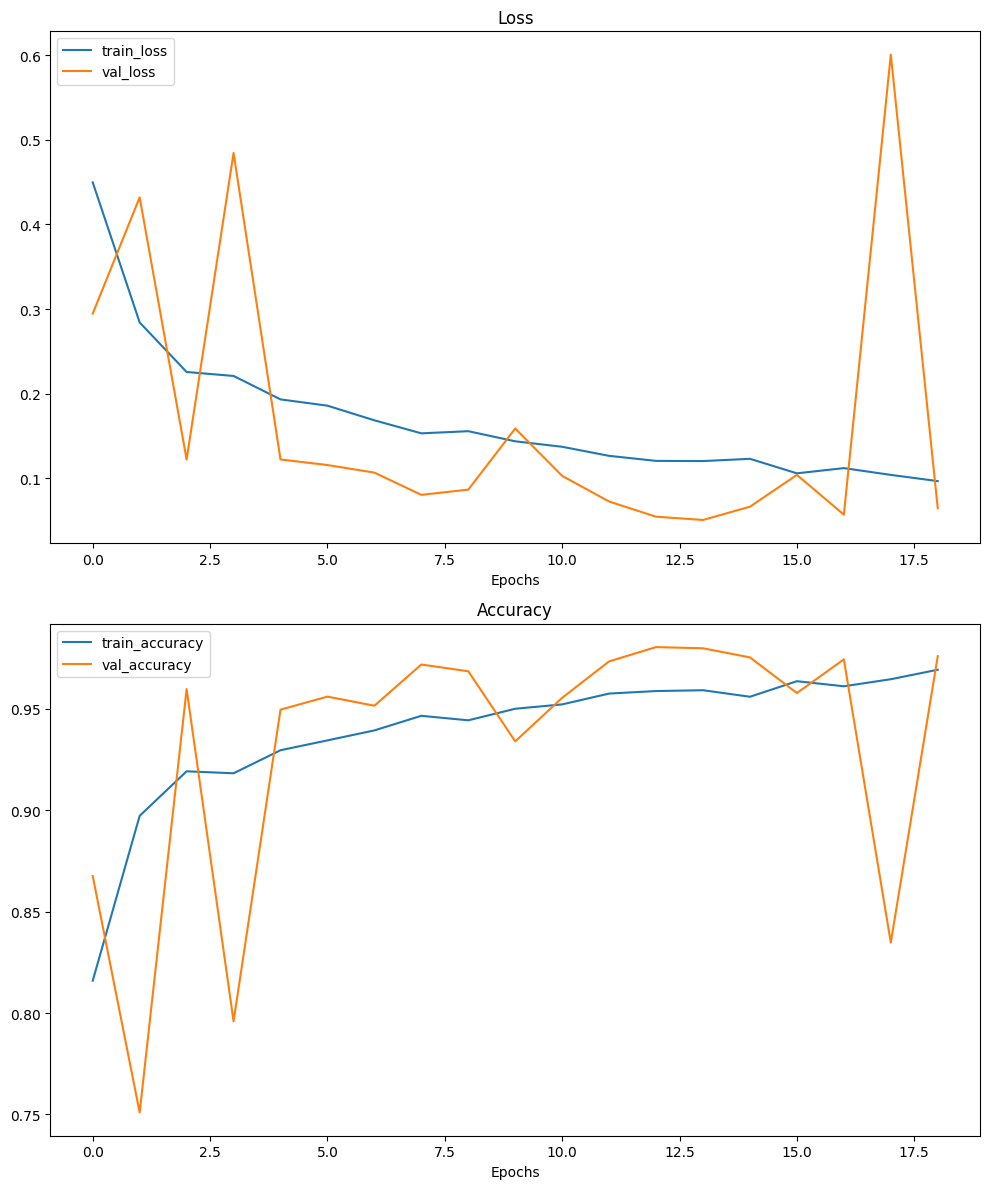
\includegraphics[width=\textwidth, height=0.9\textwidth]{imgs/cnn_train.png}
\end{figure}
\end{column}
\end{columns}
\end{frame}

\begin{frame}{ScatNet Learning Curves Analysis}
\begin{columns}[T]
\begin{column}{0.5\textwidth}
\begin{itemize}
\item \textbf{Slower convergence} but fewer epochs needed
\item \textbf{More complex classifier} needed
\item \textbf{Greater performance variation} across folds
\end{itemize}
\end{column}
\begin{column}{0.5\textwidth}
\begin{figure}
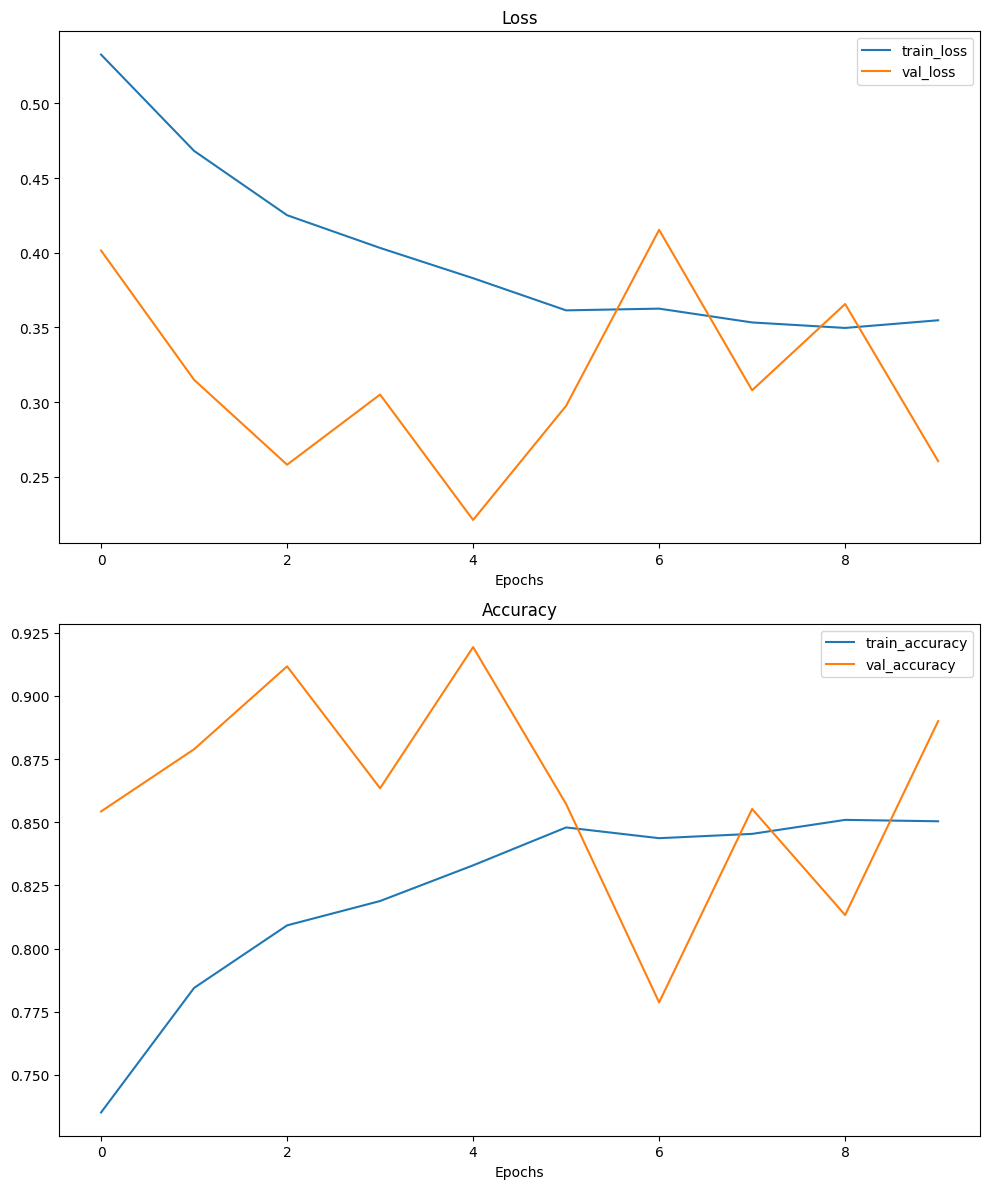
\includegraphics[width=\textwidth, height=0.9\textwidth]{imgs/scatnet_train.png}
\end{figure}
\end{column}
\end{columns}
\end{frame}

% Performance Results slide
\begin{frame}{Performance Results \& Analysis}
\begin{table}
\begin{tabular}{lll}
\toprule
Metric & CNN & ScatNet \\
\midrule
Mean Accuracy & \textbf{99.26\% ± 0.72\%} & \textbf{92.99\% ± 1.59\%} \\
Mean F1 Score & \textbf{99.27\% ± 0.72\%} & \textbf{92.83\% ± 1.70\%} \\
Accuracy Range & \textbf{97.70\% - 99.90\%} & \textbf{89.10\% - 95.10\%} \\
Training Speed & \textbf{Faster} & \textbf{Slower} \\
\bottomrule
\end{tabular}
\end{table}

\begin{block}{Key Performance Findings}
\begin{itemize}
\item CNN \textbf{significantly outperforms} ScatNet (by \textbf{6.27\%})
\item K-fold validation confirms \textbf{robust performance}
\item CNN shows \textbf{less variance} between folds
\item CNN achieves convergence in \textbf{fewer epochs}
\end{itemize}
\end{block}
\end{frame}

% Performance Summary slides
\begin{frame}{CNN Performance Summary}
\textbf{Performance Range:}
\begin{itemize}
\item Accuracy: \textbf{98.00\% - 99.90\%} across all folds
\item F1 Score: \textbf{98.01\% - 99.90\%} across all folds
\item Most consistent fold: \textbf{Fold 9} (99.90\% accuracy)
\item All folds achieved \textbf{>97.70\% accuracy}
\end{itemize}

\textbf{Overall Statistics:}
\begin{itemize}
\item Mean Accuracy: \textbf{99.26\%}
\item Mean F1 Score: \textbf{99.27\%}
\item Standard Deviation: \textbf{0.72\%}
\end{itemize}
\end{frame}

\begin{frame}{ScatNet Performance Summary}
\textbf{Performance Range:}
\begin{itemize}
\item Accuracy: \textbf{89.10\% - 95.10\%} across all folds
\item F1 Score: \textbf{88.68\% - 95.06\%} across all folds
\item Best performing fold: \textbf{Fold 6} (95.10\% accuracy)
\item Worst performing fold: \textbf{Fold 1} (89.10\% accuracy)
\end{itemize}

\textbf{Overall Statistics:}
\begin{itemize}
\item Mean Accuracy: \textbf{92.99\%}
\item Mean F1 Score: \textbf{92.83\%}
\item Standard Deviation: \textbf{1.59\%}
\end{itemize}
\end{frame}

% CNN Filter Analysis slides
\begin{frame}{CNN Filter Analysis}
\begin{columns}[T]
\begin{column}{0.6\textwidth}
\begin{itemize}
\item \textbf{Detected Filter Patterns}:
  \begin{itemize}
  \item \textbf{Diagonal/Vertical Strips}: Detect edges, gaps, and transitions between textures
  \item \textbf{Circular Points}: Identify spots, blobs, and localized features
  \item \textbf{Two-Part Filters}: Capture gradients and contrast changes
  \end{itemize}
\item \textbf{Filter Implications}:
  \begin{itemize}
  \item Learning localized and structured features
  \item Capturing directional patterns and contrast
  \item Detecting orientation-dependent structures
  \end{itemize}
\end{itemize}
\end{column}
\begin{column}{0.4\textwidth}
\begin{figure}
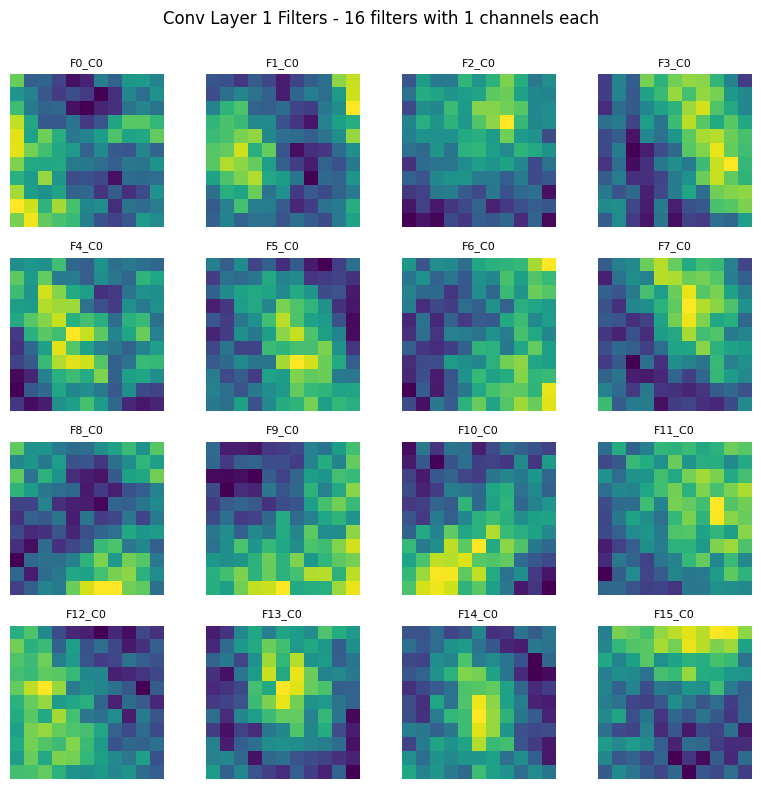
\includegraphics[width=\textwidth]{imgs/cnn_filters.png}
\end{figure}
\end{column}
\end{columns}
\end{frame}

% ScatNet Filter Analysis
\begin{frame}{ScatNet Filter Analysis}
\begin{columns}[T]
\begin{column}{0.5\textwidth}
\begin{itemize}
\item \textbf{Pre-defined wavelet transforms} (not learned)
\item \textbf{Scale and rotation invariant} features
\item \textbf{Lower discriminative power} despite theoretical advantages
\item Fixed mathematical representation \textbf{limits adaptability}
\item Data augmentation impact: \textbf{less significant}
\end{itemize}
\end{column}
\begin{column}{0.5\textwidth}
\begin{figure}
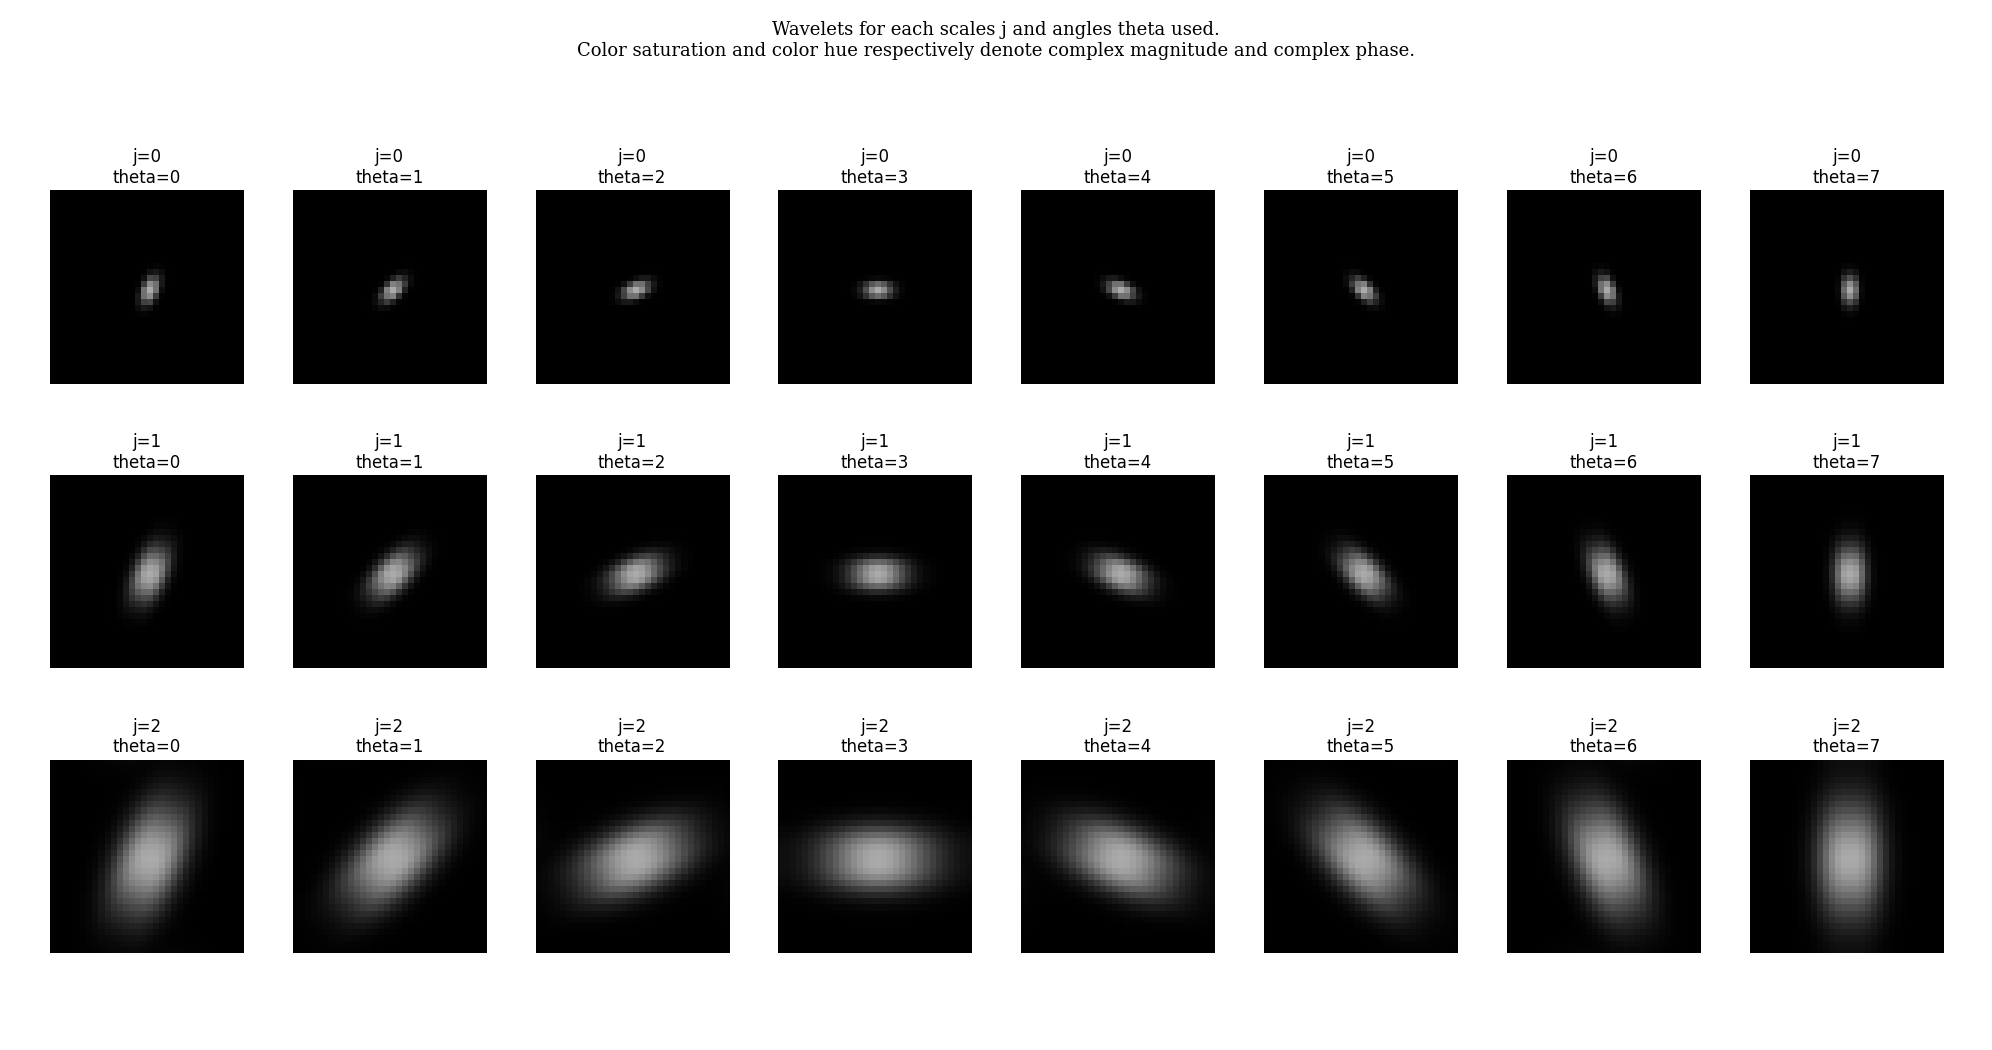
\includegraphics[width=0.7\textwidth]{imgs/scatnet_filters.png}
\vspace{0.5cm}
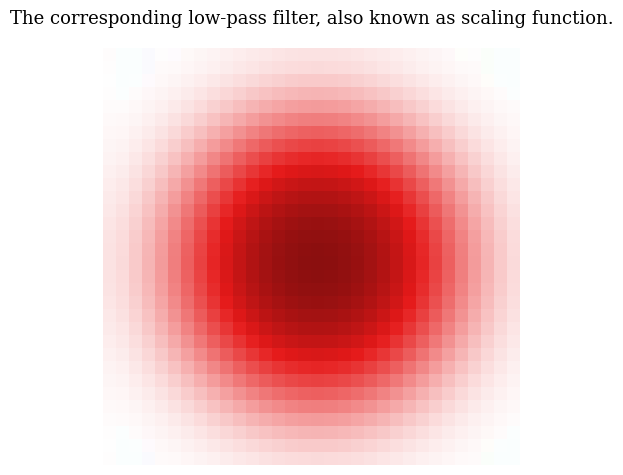
\includegraphics[width=0.7\textwidth]{imgs/scatnet_low_pass.png}
\end{figure}
\end{column}
\end{columns}
\end{frame}

% Attribution Analysis slides
\begin{frame}{CNN Attribution Analysis}
\begin{columns}[T]
\begin{column}{0.5\textwidth}
\begin{itemize}
\item Visualizes regions \textbf{most influential} for classification
\item Focuses on \textbf{cellular structures} and \textbf{patterns}
\item \textbf{Higher resolution} in feature attribution
\item \textbf{Strong correlation} with pathological markers
\end{itemize}
\end{column}
\begin{column}{0.5\textwidth}
\begin{figure}
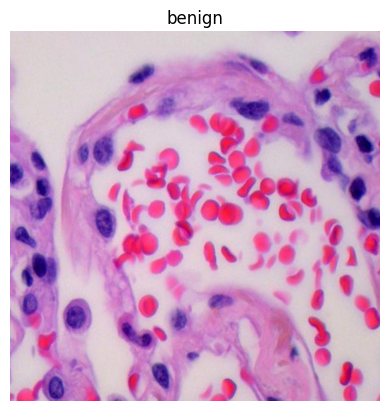
\includegraphics[width=0.45\textwidth]{imgs/normal_image.png}
\vspace{0.2cm}
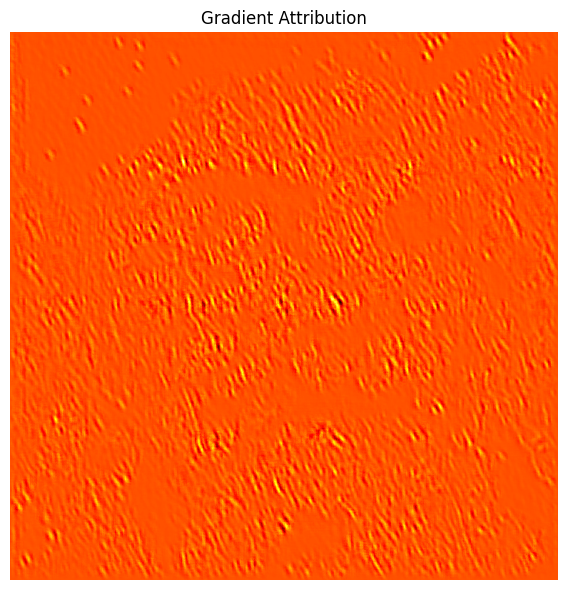
\includegraphics[width=0.45\textwidth]{imgs/cnn_bp.png}
\vspace{0.2cm}
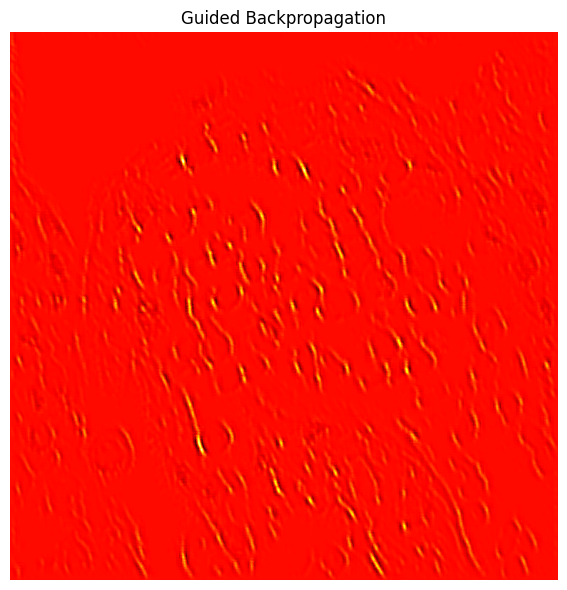
\includegraphics[width=0.45\textwidth]{imgs/cnn_gbp.png}
\vspace{0.2cm}
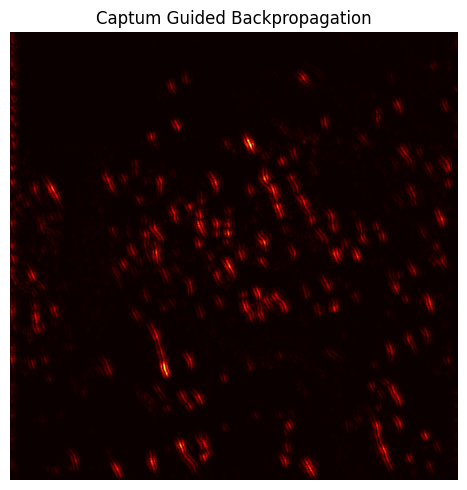
\includegraphics[width=0.45\textwidth]{imgs/cnn_gbp_captum.png}
\end{figure}
\end{column}
\end{columns}
\end{frame}

\begin{frame}{ScatNet Attribution Analysis}
\begin{columns}[T]
\begin{column}{0.5\textwidth}
\begin{itemize}
\item \textbf{Different activation patterns} compared to CNN
\item \textbf{More diffuse attribution regions}
\item Wavelets capture \textbf{texture} but miss \textbf{color information}
\item \textbf{Less aligned} with pathological indicators
\end{itemize}
\end{column}
\begin{column}{0.5\textwidth}
\begin{figure}
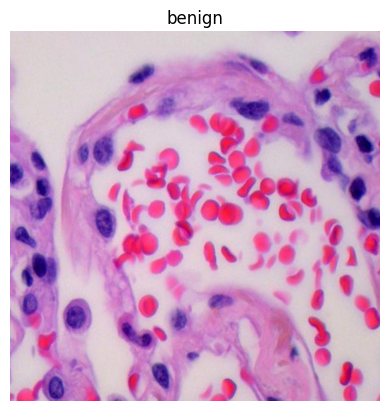
\includegraphics[width=0.45\textwidth]{imgs/normal_image.png}
\vspace{0.2cm}
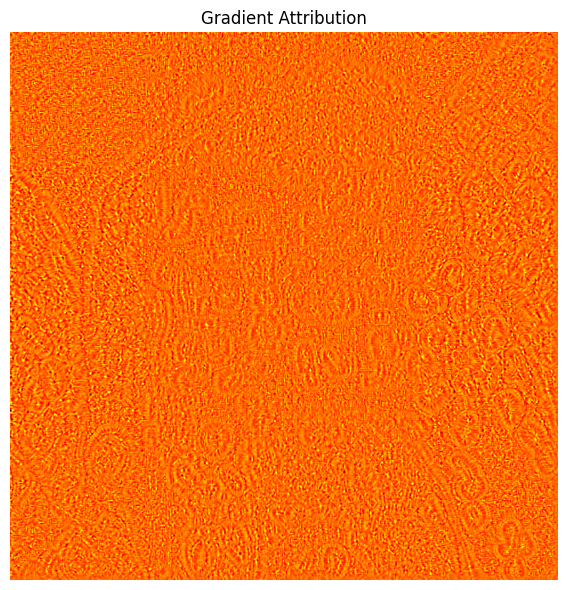
\includegraphics[width=0.45\textwidth]{imgs/scatnet_bp.png}
\vspace{0.2cm}
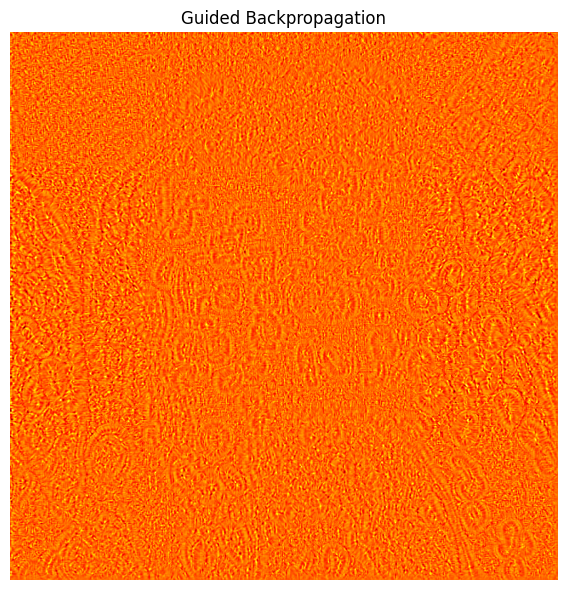
\includegraphics[width=0.45\textwidth]{imgs/scatnet_gbp.png}
\vspace{0.2cm}
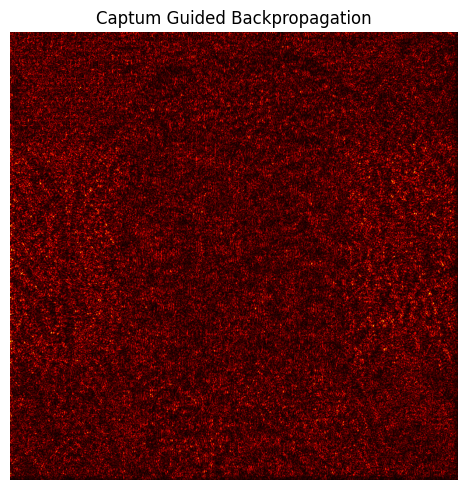
\includegraphics[width=0.45\textwidth]{imgs/scatnet_gbp_captum.png}
\end{figure}
\end{column}
\end{columns}
\end{frame}

% Implementation Comparison slide
\begin{frame}{Custom vs. Library Implementation}
\textbf{Custom Implementation:}
\begin{itemize}
\item Complete control over \textbf{visualization parameters}
\item Direct access to \textbf{gradient computation}
\item Greater understanding of \textbf{attribution mechanics}
\end{itemize}

\textbf{Captum Library:}
\begin{itemize}
\item More \textbf{visualization options} and integrated smoothing
\item \textbf{Consistent API} across different attribution methods
\item Better \textbf{computational performance}
\end{itemize}

\begin{block}{Analysis}
Both implementations highlight similar regions, \textbf{validating our approach}
\end{block}
\end{frame}

% Key Insights slide
\begin{frame}{Key Insights}
\begin{itemize}
\item \textbf{Color features} are crucial for lung cancer histopathology classification
  \begin{itemize}
  \item The class average color alone is \textbf{highly predictive}
  \end{itemize}
\item \textbf{Learned features} (CNN) outperform \textbf{fixed mathematical representations} (ScatNet)
\item \textbf{Simpler architectures} can outperform sophisticated ones when aligned with data
\item Even with grayscale images, models achieved \textbf{high accuracy}
  \begin{itemize}
  \item Focusing on \textbf{structural features} rather than just color
  \end{itemize}
\end{itemize}
\end{frame}

% Final slide
\begin{frame}[plain]
\centering
\vspace{2cm}
{\Large Thank you for your attention}

\vspace{1cm}
{\large Lorenzo Mioso}
\end{frame}

\end{document}